\documentclass[11pt]{article}
\usepackage[a4paper,margin=27mm]{geometry}
\usepackage[T1]{fontenc}
\usepackage{lmodern}
\usepackage{amsmath,amssymb,amsthm,mathtools}
\usepackage{booktabs,array}
\usepackage{microtype}
\usepackage{tikz,pgfplots}
\pgfplotsset{compat=1.18}
\usepackage[colorlinks=true,linkcolor=blue!50!black,citecolor=blue!50!black,urlcolor=blue!50!black]{hyperref}
\newtheorem{theorem}{Theorem}[section]
\newtheorem{lemma}[theorem]{Lemma}
\newtheorem{proposition}[theorem]{Proposition}
\theoremstyle{remark}
\newtheorem{remark}[theorem]{Remark}
\DeclareMathOperator{\curl}{curl}
\DeclareMathOperator{\supp}{supp}
\DeclareMathOperator{\conv}{conv}
\DeclareMathOperator{\row}{row}
\DeclareMathOperator{\vertices}{Vert}
\newcommand{\R}{\mathbb R}
\newcommand{\Z}{\mathbb Z}
\newcommand{\PP}{\mathbb P}
\newcommand{\calT}{\mathcal T}
\newcommand{\norminf}[1]{\lVert#1\rVert_\infty}
\setlength{\emergencystretch}{2em}

\title{Local potential bases on Freudenthal meshes}
\author{Kaiwen Jin\thanks{\texttt{yui.ui.siki@gmail.com}}}
\date{10 October 2026}

\begin{document}
\maketitle

\begin{abstract}
Local bases for finite-element potential spaces provide the algebraic
decompositions needed for vertex-patch corrections. On a consistently oriented
Freudenthal mesh of the cube, we prove that continuous vector polynomials of
degree $k+1$ with continuous curl have a basis supported on single vertex
stars for every $k\ge5$ and every mesh size. This establishes the local-support
assertion in the second conjecture of Farrell, Mitchell and Scott. The proof
uses exact integer certificates together with analytical arguments covering
all grids and degrees. At degree six, bounded windows transfer a fixed normal
form and two-part local repairs. At higher degrees, clipped barycentric gaps
reduce the construction to finitely many types, while affine inequalities
verify their validity over unbounded parameter regions. We also obtain an
exact dimension formula and provide reproducible basis-construction code.
The conclusion is algebraic locality; a uniform bound on decomposition norms
is a separate question.
\end{abstract}

\section{Introduction}

In a vertex-patch method, corrections act on the tetrahedra surrounding one
mesh vertex. A potential supported on such a patch has a curl supported on
the same patch, and that curl is divergence free. This gives a reason to ask
whether the entire finite-element potential space can be generated by
functions with this support. The question concerns the continuity of both a
potential and its curl, so a local basis of the ordinary continuous polynomial
space does not answer it.

Farrell, Mitchell and Scott formulate this question on uniform Freudenthal
meshes in Conjecture~2(b) of \cite[\S3.3]{FMS}. Their potential space consists
of continuous vector-valued piecewise polynomials of degree $k+1$ whose curl
is continuous. They conjecture the existence of a basis supported on vertex
stars when $k\ge5$, and give numerical evidence. We use exactly this
potential space, without imposed boundary conditions, on the six-tetrahedron
subdivision specified in their Appendix~A. Boundary vertices are included.

We prove the local-basis assertion for every integer $k\ge5$ and every
number $N\ge1$ of cubes per coordinate direction. More precisely, each
potential is a sum of potentials in the same space, each supported on one
closed vertex star. Since the space is finite dimensional, a basis can be
selected from these local generators. The construction acts on the potentials
themselves; it does not identify potentials that differ by a gradient.
Theorem~\ref{thm:main} states the result and the dimension formula.

Two different finite constructions cover the polynomial degrees. For degree
six, the coefficients and source equations of a fixed integer normal form
fit within bounded windows. Boundary distances and coordinate residues
determine which window to translate. Some canonical kernel vectors need to
be split into two local potentials. For degrees at least seven, a fixed
table describes all coefficient types. Large barycentric gaps remain
unbounded variables, and elementary affine inequalities verify every source
equation, pivot decision and support condition throughout its parameter
region. Finite checks thus establish explicit families of identities rather
than extrapolating ranks from selected meshes.

Inf-sup stability is a related but distinct issue. Ding, Ming, Yu and Zhu
prove a divergence right-inverse estimate uniform in $N$ for each fixed
velocity degree $k\ge4$, with pressure space equal to the actual divergence
image \cite[Theorem~2.1]{DMYZ}. The construction here does not use that
estimate. We prove algebraic locality without a uniform decomposition norm,
and make no claim of multigrid convergence or exactness of a discrete Stokes
complex.

Section~\ref{sec:coefficients} expresses the potential space as an integer
matrix kernel and gives the support criterion. Section~\ref{sec:uniform}
proves the uniform constructions. Section~\ref{sec:implementation} describes
the implementation, certificate verification and exact construction cases.

\section{Bernstein coefficients and local support}\label{sec:coefficients}

Let $\Omega=(0,1)^3$, $N\ge1$ and $h=1/N$. For each
$a\in h\{0,\ldots,N-1\}^3$ and permutation $\sigma\in S_3$, put
\begin{equation}\label{eq:mesh}
 T_{a,\sigma}=a+h\conv\{0,e_{\sigma_1},
                         e_{\sigma_1}+e_{\sigma_2},(1,1,1)\}.
\end{equation}
All cubes have the same orientation. The resulting mesh is $\calT_h$.
For a mesh vertex $v$, let $\omega_v$ be the union of its closed incident
tetrahedra. For an integer $d\ge6$ define
\begin{equation}\label{eq:space}
 S_{N,d}=\{w\in C^0(\overline\Omega;\R^3):
 w|_T\in\PP_d(T)^3\ (T\in\calT_h),\quad
 \curl w\in C^0(\overline\Omega;\R^3)\}.
\end{equation}
Here $\PP_d$ denotes total degree at most $d$, and the curl is initially
taken on each polynomial piece. No condition is imposed on a physical
boundary face. Support is closed support in $\overline\Omega$.

\begin{theorem}\label{thm:main}
For every integer $N\ge1$ and $d\ge6$, the real vector space $S_{N,d}$
has a basis each of whose members is supported in a single $\omega_v$.
Equivalently,
\begin{equation}\label{eq:decomposition}
 S_{N,d}=\sum_v\{w\in S_{N,d}:\supp w\subseteq\omega_v\}.
\end{equation}
For $N\ge2$ its dimension is
\begin{equation}\label{eq:dimension}
 3N^3(d-1)^2(d-2)+3N^2(d-1)(5d-4)+9N(2d-1)+6.
\end{equation}
At $d=6$ this formula also holds for $N=1$.
\end{theorem}

With $d=k+1$, the dimension in \eqref{eq:dimension} is
$3N^3k^2(k-1)+3N^2k(5k+1)+9N(2k+1)+6$. The support assertion
includes all $N\ge1,k\ge5$. We prove the theorem in
Section~\ref{sec:uniform} by constructing matrix kernels with actual
vertex-star support.

\subsection{A global coefficient lattice}

Use the scaled coordinates $y=Nx$, so mesh cells have side length one.
The polynomial degree and support do not change, and
$\curl_x=N\curl_y$. On an ordered tetrahedron with vertices
$v_0,\ldots,v_3$ in the scaled mesh, let $\lambda_i$ be its barycentric
coordinates. Its degree-$d$ Bernstein polynomials are
\[
 B^d_\alpha=\frac{d!}{\alpha_0!\cdots\alpha_3!}
             \prod_{i=0}^3\lambda_i^{\alpha_i},
 \qquad \alpha_i\in\Z_{\ge0},\quad |\alpha|=d.
\]
They form a basis of $\PP_d$: homogenizing any lower-degree monomial by
$(\sum_i\lambda_i)^{d-r}=1$ proves spanning, and their number
$\binom{d+3}{3}$ equals the polynomial-space dimension. On a face opposite
$v_j$, exactly the terms $\alpha_j=0$ remain and form its face Bernstein
basis. Equality of traces is therefore equality of those coefficients.

Label a coefficient by
\begin{equation}\label{eq:q}
 q=\sum_{i=0}^3\alpha_i v_i\in\Lambda_{N,d}:=\{0,\ldots,Nd\}^3.
\end{equation}
This is a coefficient label, not evaluation at $q/d$. To recover its
canonical tetrahedron, set
\begin{equation}\label{eq:canonical}
 a_j=\min(\lfloor q_j/d\rfloor,N-1),\qquad r_j=q_j-da_j.
\end{equation}
Sort $r$ in decreasing order, breaking ties by increasing coordinate index,
to obtain $\sigma$. The local multiindex is
\begin{equation}\label{eq:gaps}
 \alpha=(d-r_{\sigma_1},\ r_{\sigma_1}-r_{\sigma_2},\
                r_{\sigma_2}-r_{\sigma_3},\ r_{\sigma_3}).
\end{equation}
It is nonnegative and sums to $d$, proving that every label in
$\Lambda_{N,d}$ occurs.

The vertices with positive $\alpha_i$ span the unique mesh entity $E(q)$
whose relative interior contains $q/d$. Every occurrence of $q$ is the
coefficient of that same entity, with its face-trace identification.
Incident tetrahedra of an entity are connected through faces containing
it, including at the boundary. Indeed, a sufficiently small ball about a
relative-interior point meets only simplices containing that point.
Its intersection with the cube is convex. Generic polygonal paths between
incident tetrahedron interiors cross full faces and avoid the finite
collection of lower-dimensional intersections. This gives the claimed
connection. Consequently the trace identifications give precisely one
scalar coefficient per $q$. Continuous vector polynomials are parametrized
by $c=(c_{q,j})$, $j=1,2,3$, with ambient dimension
\begin{equation}\label{eq:ambient}
 n=3(Nd+1)^3.
\end{equation}

\subsection{Curl continuity and support}

On a chain tetrahedron in scaled coordinates the barycentric gradients are
\begin{equation}\label{eq:gradients}
 g_0=-e_{\sigma_1},\quad g_1=e_{\sigma_1}-e_{\sigma_2},\quad
 g_2=e_{\sigma_2}-e_{\sigma_3},\quad g_3=e_{\sigma_3}.
\end{equation}
Differentiation of the Bernstein expansion gives
\begin{equation}\label{eq:curl}
 d^{-1}\curl_y w
   =\sum_{|\beta|=d-1}B^{d-1}_\beta
      \sum_{i=0}^3g_i\times c_{\sum_m\beta_m v_m+v_i}.
\end{equation}
For an internal face and its degree-$(d-1)$ face multiindex $\beta$,
subtract the two inner sums in \eqref{eq:curl}. The three Cartesian
components give integer rows of a matrix $A_{\rm all}$; its entries are
$0,\pm1,\pm2$. Physical faces give no rows. Equal face traces also match
curl values at edges and vertices by the preceding adjacency argument.
Thus the coefficient representation identifies
\begin{equation}\label{eq:kernel}
 S_{N,d}\simeq\ker_\R A_{\rm all}.
\end{equation}

Two components suffice on each internal face. For a continuous vector
polynomial, the jump of each component's gradient is parallel to the face
normal $\nu$. Writing these multiples as a vector $b$, the curl jump is
$\nu\times b$, perpendicular to $\nu$. This polynomial identity holds
for each face coefficient. If $\nu_t\ne0$, the $t$th component is
$-\sum_{j\ne t}(\nu_j/\nu_t)$ times the others. The normal may be chosen
from \eqref{eq:gradients}, with nonzero components $\pm1$. The matrix $A$
obtained by omitting the first nonzero-normal component on each face
therefore has the same real row space as $A_{\rm all}$. Degree-six
certificates use $A$; higher-degree certificates verify all components.

For a label $q$, let $I(q)$ be the incident tetrahedra of $E(q)$ and put
$J(q)=\bigcap_{T\in I(q)}\vertices(T)$. A nonzero Bernstein coefficient
makes the polynomial nonzero in every such tetrahedron, by local
independence. Its support includes the closure of each of those interiors.
It follows that
\begin{equation}\label{eq:support}
 \supp w\subseteq\omega_v
 \quad\Longleftrightarrow\quad
 v\in\bigcap_{c_{q,j}\ne0}J(q).
\end{equation}
In particular, $v\in\vertices(E(q))$ at each nonzero coefficient is sufficient.
It is not asserted necessary: $J(q)$ may be larger on the boundary.

\subsection{A normal form for the kernel}

\begin{lemma}\label{lem:normalform}
Suppose $C$ has $r$ rows and $n$ columns, an ordered set of columns $P$
satisfies $C[:,P]=I_r$, and $\row C=\row A$. If $F$ is the complementary
set of columns, then
\begin{equation}\label{eq:gf}
 g_f=e_f-\sum_{p\in P}C_{p,f}e_p,\qquad f\in F,
\end{equation}
is a basis of $\ker_\R A$, of dimension $n-r$.
\end{lemma}
\begin{proof}
The equations $Cc=0$ are $c_P=-C[:,F]c_F$. Free coordinates are arbitrary
and determine $c$ uniquely. The vectors \eqref{eq:gf} have the identity
matrix in these coordinates, proving independence and spanning.
\end{proof}

If every $g_f$ is a sum of local vectors in the kernel, their combined
parts form a finite local spanning set. Successively retain vectors
independent of those already retained; the resulting subset is a local
basis. For a small finite case we also use this elementary rank criterion:
if integer matrices $A,B$ satisfy $AB^T=0$, $A$ has a nonzero $r$-minor
modulo a prime, $B$ has a nonzero $s$-minor modulo that prime, and $r+s=n$,
then $B$ is a real kernel basis. The nonzero modular determinants are
nonzero integers, giving real rank lower bounds; membership supplies the
opposite dimension inequality. No equality of modular and real ranks is
assumed.

\section{Uniform constructions}\label{sec:uniform}

\subsection{Degree six: bounded windows and local repairs}

For this subsection $d=6$. The reference grid has $N=6$. Reassembling
the integer curl matrix gives a fixed certificate $W,C,P$ satisfying
\begin{equation}\label{eq:six-identities}
 C=WA,\qquad A=A[:,P]C,\qquad C[:,P]=I.
\end{equation}
Here $n=151959$, $|P|=72519$, and there are $79440$ free columns.
Define the window signature
\begin{equation}\label{eq:eta}
 \eta_R(q;N)=\big((q_j\bmod6,\min(q_j,R+1),
                              \min(6N-q_j,R+1))\big)_{j=1}^3.
\end{equation}
Distances and radii in this subsection refer to the coefficient lattice,
so a scaled mesh vertex $v$ is at coefficient position $6v$.

The following finite properties are verified for every row or column of
the reference certificate. Section~\ref{sec:verification} specifies the
checks and their arithmetic.
\begin{enumerate}
\item The pivot/free decision, and the relative $C$ row at a pivot,
depend only on $(\eta_5(q;6),j)$. There are $17496=3\cdot18^3$ such
decisions. Every nonzero coefficient of the row is within distance seven
of its pivot in the infinity norm.
\item Every nonzero original row has its coefficients within distance two
of its first coefficient position. The vertices of both incident
tetrahedra lie within distance seven. For a source row used in $C_p=W_pA$,
both full tetrahedra lie within distance eleven of the pivot.
\item Of the canonical vectors \eqref{eq:gf}, $78715$ have a recorded
single-star owner. Each of the other $725$ is the sum of two saved local
kernel vectors. The $1450$ repair parts have integer coefficients of
magnitude at most two, and the sums have denominator one.
\item For every recorded owner $v$ of a vector or a repair part anchored
at free column $f$, $\norminf{6v-q_f}\le6$. Every vertex of its entire
star lies within coefficient distance twelve of $q_f$.
\end{enumerate}
The second property bounds the complete source geometry, which is stronger
than bounding the positions of its nonzero coefficients.

\begin{lemma}\label{lem:windows}
For $N\ge5$ and $R\in\{5,7,11,12\}$, every signature $\eta_R(q;N)$
that occurs has a representative on $N=6$. Their anchors differ by a
vector in $(6\Z)^3$. Translation identifies the mesh and its physical
boundary within radius $R$. If two anchors have the same $\eta_{R+s}$,
every shift of infinity norm at most $s$ has the same domain-membership
decision and, when inside, the same $\eta_R$ at both anchors.
\end{lemma}
\begin{proof}
In one coordinate the left and right bands of width $R$ are disjoint,
since $6N\ge30>2R$. A point in the left band is represented by the same
integer on $[0,36]$; distance $t\le R$ from the right boundary is
represented by $36-t$. For an interior point, the reference interval
$[R+1,35-R]$ contains all six residues. Residue equality makes the
translation divisible by six. The exact distances identify each visible
boundary plane; clipped distances put the others outside the window.
For a shift of size at most $s$, a boundary at distance at most $R+s$
has its distance recorded exactly. A boundary farther away cannot enter
the radius-$R$ shifted window. Residues change by the same shift.
Apply this argument to each coordinate.
\end{proof}

Only occurring target signatures need representatives. At $N=5,R=12$
the interior interval contains five positions, so requiring all six
residues there would be incorrect.

For any $N\ge5$, define $P_N$ and $C_N$ by the reference $\eta_5$ table.
To prove the forward inclusion, choose a reference pivot with the same
$\eta_{11}$. Every source face and both adjacent tetrahedra in its
identity $C_p=W_pA$ translate by Lemma~\ref{lem:windows}. Their equations
and weights are unchanged, proving $\row C_N\subseteq\row A_N$.

For the reverse inclusion, anchor an original nonzero row at its first
coefficient and choose a reference with the same $\eta_7$. This preserves
the full row geometry. Each of its coefficient positions is within
distance two, so its $\eta_5$ and pivot/free status are preserved.
The relative $C$ row at each pivot is therefore the same. The reference
identity $a=a[:,P]C$ translates term by term, proving
$\row A_N\subseteq\row C_N$. Finally choose $\eta_{12}$ at a pivot:
the radius-seven row and radius-five decisions at its coefficients agree
with the reference. Thus its only pivot coefficient is one at the
anchor, and $C_N[:,P_N]=I$. Lemma~\ref{lem:normalform} gives a canonical
kernel basis for every $N\ge5$.

A canonical vector $g_f$ depends on $\eta_{12}(q_f;N)$ and component.
Indeed all its pivot coefficients are within distance seven of $f$;
their radius-five decisions and relative rows determine its entire
pattern. Choose a reference free vector with that signature. If it is
local, translate it and its owner; otherwise translate its two repair
parts. Their complete owner stars fit within radius twelve and are
matched by Lemma~\ref{lem:windows}.

For a translated part, continuity inside the star follows from the
reference face equations. At an internal face separating the star from
its exterior, both the potential trace and curl trace of the reference
part are zero, since its exterior polynomial is zero. Translation
preserves the inside tetrahedron, that face, and whether it is physical.
Extension by zero outside the target star therefore preserves both
continuities. The exterior tetrahedron need not be in the window: only
the inside traces must be transported. Face connectivity gives continuity
at edges and vertices as well. The repair sums remain exact equalities
of potentials. These local vectors span every $g_f$, giving a local basis.

The small grids are handled by exact integer certificates and the minor
criterion above. At $N=1,2,3,4$ the basis dimensions are respectively
$795,4164,11913,25842$. Each basis has zero integer curl residual and
nonempty support intersections. Modulo $1000003$, the prescribed constraint
minors are $-1$, and the prescribed basis minors are $1,1,-1,1$,
respectively. Their orders sum to the ambient dimension.

For $N\ge5$, count the free $\eta_5$ types. Each boundary distance
$0,\ldots,5$ occurs once at each end. In the interior interval
$[6,6N-6]$, residue zero occurs $N-1$ times and every other residue
$N-2$ times. Multiplying the coordinate multiplicities and summing the
free types gives the exact polynomial
\begin{equation}\label{eq:six-dimension}
 \dim S_{N,6}=300N^3+390N^2+99N+6.
\end{equation}
The small-grid dimensions satisfy the same formula. This proves the
degree-six part of Theorem~\ref{thm:main}.

\subsection{Higher degrees: unbounded gap parameters}

Here $N\ge2,d\ge7$. Use the canonical cell and gaps in
\eqref{eq:canonical}--\eqref{eq:gaps}. The cell boundary class $b_j$ is
zero for the first cell, two for the last, and one otherwise. Put
$\gamma_i=\min(\alpha_i,3)$ and define the coefficient type
\begin{equation}\label{eq:type}
 \tau=(b,\sigma,\gamma,j),\qquad j\in\{1,2,3\}.
\end{equation}
For $\gamma_i<3$ the gap is fixed to that integer; a value three means
the unbounded variable $\alpha_i\ge3$. Always $\sum_i\alpha_i=d\ge7$.

The feasible types are determined exactly by three conditions. If there
is no tail, $\sum_i\gamma_i\ge7$. A zero intervening gap requires the
tied consecutive ordering indices to increase. If $\gamma_0=0$, all
leading coordinates whose remainder is $d$ must be in a last cell.
These conditions are necessary from the canonical rule. Conversely,
choose the fixed gaps and tails, increasing a tail if needed to reach
degree seven, and place the cell classes on $N=3$. Reconstruct the
remainders from the gaps. The tie conditions give the canonical order,
and the last-cell condition makes every remainder equal to $d$ valid.
This realizes the type. Enumeration gives $59943$ feasible types, and
the rule table is checked to have exactly this set of keys.

The table declares $17331$ pivot types and $42612$ free types. Each pivot
has a fixed integer relative row, with coefficient magnitude at most three
and position offsets at most seven, and explicit source face equations.
To verify these formulas over all degrees we use the following elementary
minimum rule.

\begin{lemma}\label{lem:affine}
Let each integer $x_i$ be fixed to $\ell_i$ or range over $x_i\ge\ell_i$,
with $\sum_i x_i\ge s$. On a nonempty such region, an affine form
$L=c_0+\sum_i c_ix_i$ is unbounded below if a variable coefficient is
negative. Otherwise its minimum is
\begin{equation}\label{eq:affine-min}
 c_0+\sum_i c_i\ell_i+
       \max(0,s-\sum_i\ell_i)\min_{i\text{ variable}}c_i.
\end{equation}
If all coordinates are fixed, evaluate at that single feasible point.
An affine identity holds throughout the region exactly when all variable
coefficients vanish and the value at a feasible point is the desired constant.
\end{lemma}
\begin{proof}
Write $x_i=\ell_i+t_i$. Variable $t_i$ are nonnegative and can increase
independently. A negative coefficient makes $L$ tend to $-\infty$.
For nonnegative coefficients, place the required excess
$\max(0,s-\sum\ell_i)$ entirely in a variable with least coefficient;
this attains the lower bound. Independent increases also prove the
identity criterion.
\end{proof}

\paragraph{Forward row identities.}
Write $(R_\sigma\alpha)_{\sigma_i}=\sum_{t=i}^3\alpha_t$ for
$i=1,2,3$, so $q=da+R_\sigma\alpha$. A source record lists two chain
tetrahedra relative to $a$, their common face, an offset $\delta$, a curl
component and an integer weight. Each tetrahedron must have the three
distinct positive coordinate steps and the listed face must be exactly
their three-vertex intersection. Its relative vertices obey coordinate
bounds $[0,2]$ in a first cell, $[-1,2]$ in an interior cell, and
$[-1,1]$ in a last cell. These bounds keep the source in the physical
mesh for all $N\ge2$ in that context.

Write its relative barycentric functions as
$\lambda_i(z)=\ell_i+g_i\cdot z$. The source's face multiindex at
$(d-1)a+R_\sigma\alpha+\delta$ is
\begin{equation}\label{eq:source-beta}
 \beta_i=\ell_i(d-1)+g_i\cdot(R_\sigma\alpha+\delta).
\end{equation}
Lemma~\ref{lem:affine} checks that the opposite coordinate is identically
zero and the three face coordinates are nonnegative throughout the type's
unbounded region. They sum to $d-1$ since $\sum\ell_i=1$ and
$\sum g_i=0$. Each source is therefore an actual face equation for
every admissible degree. Substituting \eqref{eq:curl} and the integer
weights must give the declared row exactly, after summing duplicate
offsets. All $105320$ sources satisfy these checks, including $631920$
nonnegativity inequalities and $210640$ plane identities. This proves
$\row C\subseteq\row A_{\rm all}$ for the matrix obtained by applying
the table at each coefficient site.

\paragraph{Shifted types and pivots.}
For a row of offset radius $\rho\le7$, set
$M=\max(7,2\rho+3)\le17$. Partition every tail into the alternatives
$\alpha_i=3,\ldots,M-1$ and $\alpha_i\ge M$, retaining
$\sum\alpha_i\ge7$ and discarding empty regions. For a shifted site
$q'=q+\delta$, classification at a feasible representative proposes its
cell $a'$, order and clipped gaps. The proposal is then proved throughout
the region by Lemma~\ref{lem:affine}, checking
\begin{align*}
 &0\le q'_j\le Nd,\qquad r'_j=q'_j-da'_j\ge0,\\
 &d-r'_j\ge1\quad(a'_j<N-1),\qquad d-r'_j\ge0\quad(a'_j=N-1).
\end{align*}
Consecutive remainders must be nonincreasing, with a difference at least
one when their indices are decreasing. A proposed gap below three must
be identically that integer; a tail must be at least three everywhere.
Thus a representative is never used as a substitute for a uniform check.

Since $\rho\le7\le d$, a shifted canonical cell differs by at most one
per coordinate. For $N\ge4$, first, second, distant interior, penultimate
and last cells represent all possible boundary contexts. They are realized
on $N=5$ at positions $0,1,2,3,4$; $N=4$ simply lacks the distant
case. The boundary status of every one-cell shift is preserved. The
overlapping contexts for $N=2,3$ are processed directly. Cartesian
products of these contexts cover all grids.

Every checked off-diagonal entry is at a free type, and the only pivot
entry of each row is one at its anchor. The finite traversal covers
$249177$ parameter regions, $1569530$ grid-context regions and
$10782184$ off-diagonal links. This proves $C[:,P]=I$ uniformly.

\paragraph{Vertex owners.}
The positive-gap vertices of the canonical tetrahedron are $E(q)$; their
identity depends only on $\sigma,\gamma$. Start the owner mask of a
free type with these vertices, expressed as the eight binary vertices of
its canonical cube. For every link $C_{p,f}\ne0$, intersect that mask
with $\vertices(E(q_p))$ expressed relative to the free site's cell.
Intersect over all regions and all boundary contexts just described.
Every possible link is covered, and all $42612$ free-type masks remain
nonempty. A surviving vertex belongs to $E(q_f)$ and every $E(q_p)$
occurring in $g_f$. Choosing its least bit gives a mesh vertex $v_f$.
The sufficient condition in \eqref{eq:support} proves
$\supp g_f\subseteq\omega_{v_f}$ for every grid and degree.

\paragraph{Reverse row identities.}
For an internal face and its two tetrahedra let $o$ be their coordinatewise
minimum and let $w_j$ be their coordinate widths. The tets occupy one cube
or two cubes sharing a square face, so $w_j\in\{1,2\}$. Record the
relative face and tetrahedron vertices and the boundary information
\begin{equation}\label{eq:face-profile}
 (\mathbf1_{o_j=0},\min(N-o_j-w_j,2))_{j=1}^3.
\end{equation}
Enumeration on $N=2,\ldots,6$ gives exactly $888$ distinct profiles,
and a set comparison verifies the file against that enumeration. This
covers every $N$: for $N\ge6$ map each origin coordinate to $N=6$ by
\[
 o'_j=\begin{cases}
 0,&o_j=0,\\
 6-w_j,&N-o_j-w_j=0,\\
 5-w_j,&N-o_j-w_j=1,\\
 1,&\text{otherwise}.
 \end{cases}
\]
When $o_j=0$ its upper distance is at least four, so the first case
preserves both clipped distances. All other cases preserve the lower
flag and the upper distance class. Smaller grids were enumerated directly.

Let the face multiindex be $\beta=(\beta_0,\beta_1,\beta_2)$, with
$d=1+\sum\beta_i\ge7$. If $f_i$ and $t_j$ are relative face and
tetrahedron vertices, an original row coefficient occurs at
\begin{equation}\label{eq:face-site}
 q=do+\sum_i\beta_i f_i+t_j.
\end{equation}
Its position $q/d$ is a convex combination of actual vertices. Its
canonical cell lies within the two tetrahedra's bounding box; profile
\eqref{eq:face-profile} consequently preserves whether that cell is first,
interior or last, including upper-plane coefficients assigned to the last
cell. Relative remainders and ordering are preserved by cell translation.

Partition each $\beta_i$ into $0,1,2,3,4$ and the unbounded tail
$\beta_i\ge5$, retaining $\sum\beta_i\ge6$. On every feasible region,
classify all nonzero columns of every Cartesian curl row using the
uniform affine tests. Subtract the appropriate $C$ row at each pivot
column, with multiplier equal to that original coefficient. Store the
residual by relative coefficient offset and component, subtracting the
common moving face position. Each residual is the empty integer
dictionary. Hence the exact identity
\begin{equation}\label{eq:reverse}
 a=a[:,P]C
\end{equation}
holds throughout each region. The checks cover $144744$ regions,
$358926$ nonzero row identities and $1713456$ coefficient classifications.
Zero original rows are automatic identities. All three curl components
are included. We obtain $\row A_{\rm all}\subseteq\row C$ for all
$N\ge2,d\ge7$.

The forward and reverse identities and unit pivot block now give a kernel
basis by Lemma~\ref{lem:normalform}. The owner intersections prove that
each member is supported on one vertex star. This proves the support
part of Theorem~\ref{thm:main} in the higher-degree range.

\subsection{Counting and completion of the theorem}

For a free type, let $b$ be the number of interior cell-coordinate classes,
$m$ the number of tail gaps, and $s=\sum_i\gamma_i$. Its cell multiplicity
is $(N-2)^b$. For $m>0$ the number of gap choices at degree $d$ is
\[
 \binom{d-s+m-1}{m-1}\quad(d\ge s),
\]
and zero otherwise: write each tail as $3+t_i$ and distribute $d-s$
nonnegative units. For $m=0$ the multiplicity is one if $d=s$ and zero
otherwise. Canonical classification makes this a bijective count.

All lower sums are at most twelve, and types without tails have sum at
most eight. For $d\ge12$ the dimension is therefore the polynomial
\begin{equation}\label{eq:count}
 \sum_{\tau\text{ free},\ m>0}
 (N-2)^b\frac{\prod_{t=1}^{m-1}(d-s+t)}{(m-1)!}.
\end{equation}
Exact rational expansion of the fixed table gives
\eqref{eq:dimension}. For $d=7,\ldots,11$, the binomial/indicator
sum is checked as an exact polynomial in $N$ to give the same formula;
$d=12$ is checked at the transition as well. Equation
\eqref{eq:six-dimension} supplies degree six.

\begin{proof}[Completion of Theorem~\ref{thm:main}]
The degree-six window construction, including the four small-grid
certificates, proves \eqref{eq:decomposition} for all $N$ at $d=6$.
The gap construction proves it for $N\ge2,d\ge7$. If $N=1$, every
tetrahedron contains $(0,0,0)$, whose star is the whole cube. The space
is finite dimensional, so any basis proves the remaining cases. Selecting
an independent subset of local generators preserves support. The counts
above prove the stated dimension ranges. Finally $y=Nx$ preserves support
and both continuities, completing the physical-domain statement.
\end{proof}

\section{Implementation and exact experiments}\label{sec:implementation}

\subsection{Basis construction}

The accompanying Python package stores each basis member as a row of
integer vector Bernstein coefficients. Its input is $N\ge1,d\ge6$;
the output is a sparse basis matrix $B$, one owner vertex per row,
and, when available, the normal form and pivot/free columns. Certificate
files are verified against their SHA-256 manifest before use. Components
are indexed from zero in the code, with increasing-index tie breaks as above.

\begin{center}
\begin{minipage}{.96\textwidth}
\hrule\smallskip
\textbf{Algorithm 1. Local potential basis construction}\par\smallskip
\begin{tabbing}
\quad\=\quad\=\quad\=\kill
\textbf{Input:} integers $N\ge1,d\ge6$; fixed certificate tables.\\
\textbf{Output:} $B\in\Z^{D\times n}$ and $D$ owner vertices.\\
Build the mesh, lattice labels and local Bernstein maps; $n=3(Nd+1)^3$.\\
\textbf{if} $d=6$ and $N<5$:\\
\>Load the finite local basis and compute its support intersections.\\
\textbf{else if} $d=6$:\\
\>Apply the $\eta_5$ table to all $n$ coefficients; form $C,P,F$.\\
\>Form each $g_f$ by \eqref{eq:gf}; choose its $N=6$ representative by $\eta_{12}$.\\
\>Keep a local $g_f$, or replace it by its two translated repair parts.\\
\>Select independent rows using exact elimination modulo $1000003$.\\
\textbf{else if} $N\ge2$:\\
\>\textbf{for each} coefficient $(q,j)$, classify $\tau$ and append its fixed row or free index.\\
\>Form $B$ from \eqref{eq:gf}; assign each free type's least owner-mask bit.\\
\textbf{else}:\\
\>Compute an integer kernel on the one-cube grid; assign owner $(0,0,0)$.\\
Reassemble all three curl components and require $A_{\rm all}B^T=0$.\\
Check every recorded owner, independence and the applicable dimension count.\\
Return the checked sparse rows and owner vertices.
\end{tabbing}
\smallskip\hrule
\end{minipage}
\end{center}

For $N\ge2,d\ge7$, construction requires $O(n)$ coefficient operations
and storage in a unit-cost model with constant-time lattice addressing.
The type table and maximum offsets are fixed. Each canonical vector
contains only sites within radius seven, so its number of coefficients
is bounded independently of $N,d$. The explicit tetrahedral Bernstein
map has $6N^3\binom{d+3}{3}=O(n)$ entries. The implementation uses
dictionary addressing, for which this cost is expected rather than a
worst-case hash bound. These estimates exclude full certificate replay
and bit complexity of arbitrarily large indices.

At degree six, translating the local generating family also has $O(n)$
size. The independent-subset selection may create fill during elimination;
we do not assign it the same linear cost. A dense worst-case bound is
$O(D^3)$ arithmetic and $O(D^2)$ workspace for the projected generator
matrix, where $D=\dim S_{N,6}$ and there are at most $2D$ generators.
Because each canonical vector is an integral sum of those generators,
their free-coordinate projections span modulo any prime. Nonzero modular
minors imply real independence, while exact integer membership is checked
separately. The one-cube implementation uses modular elimination with a
rational lift and accepts it only after exact membership and complementary
rank bounds; unsuccessful reconstruction raises an error.

The package checks integer accumulation bounds before sparse products
and raises an error rather than allowing possible overflow. Pointwise
potential and physical-curl evaluation uses floating-point Bernstein
formulas and is tested separately against a global polynomial field.
No conditioning or numerical-stability theorem is asserted for evaluation.

\subsection{Finite witness verification}\label{sec:verification}

The proof's fixed witnesses accompany the submission package
\emph{AIM 633: Local potential bases on Freudenthal meshes}, version 0.1.0.
The directory \path{src/freudenthal/certificates/} contains
\path{all_degree_rules.json.gz} and \path{verification_data.zip},
with respective SHA-256 hashes:
\begin{center}\small\ttfamily
43d45cfd9394befe130b7e5e27f22851369e0adaf0669f8526e3d8156bc7b5ee\\
32c3c6847241288a4607d699e68ac7fbbdae3378e4057531c44a94274f85f7c7
\end{center}
The release manifest verifies these files and the ZIP's member manifest
identifies every extracted witness. From the installed repository, run
\texttt{python verify\_all.py} to replay the checks in a fresh local result
directory. These are essential proof data, distinct from the larger generated
bases. The verification scripts check the following statements directly:
\begin{enumerate}
\item Degree six: reconstruct the matrices; verify all identities in
\eqref{eq:six-identities}; traverse every relative normal-form signature;
bound complete source geometries; reconstruct the canonical vectors;
check every repair's membership, owner star and exact sum; verify the
four prescribed small-grid minors.
\item Higher degrees: compare rule keys with the complete feasible-type
set; prove source admissibility using \eqref{eq:source-beta}; verify exact
integer source sums; traverse all gap and boundary contexts for the unit
pivots and owner intersections; compare the face-profile set with its
geometry enumeration and verify \eqref{eq:reverse} on every unbounded
face-parameter region.
\item Count the free types using exact rational polynomial arithmetic,
including the transition degrees. Independently reassemble degree-six
matrices with the analytical gradients \eqref{eq:gradients}.
\end{enumerate}
The normal-form discovery code and recovered rank observations are not
needed to accept any of these predicates.

Python geometry, source and affine checks use exact integers; dimension
expansion uses exact rationals. Sparse products are evaluated as bounded
integer sums. The C++ affine checker uses signed 64-bit integers and
is compiled with undefined-behavior sanitization. It evaluates bounded
affine representatives, not an unbounded actual degree. In the pivot
checks each representative gap is at most seventeen and the degree at
most sixty-eight; reference grids have at most six cells per axis.
Classification-form coefficients are bounded by twenty and their
evaluations by two thousand. Even the permitted input bounds of $1000$
row terms and coefficient magnitude $1024$ give a conservative residual
accumulation bound $16\cdot2\cdot1000\cdot1024<2^{63}-1$. The fixed
run's loop counters are below $10^9$. Python integer arithmetic checks
the JSON-to-integer table export before the C++ traversal.

These checks form a computer-assisted proof using an inspected program,
integer arithmetic libraries, compiler and hardware as its trusted computing
base. The analytical window and parameter-coverage arguments establish
why the finite traversals cover all $N,d$. The work is not a proof-assistant
formalization.

\subsection{Construction cases and a sparsity diagnostic}

Table~\ref{tab:cases} reports ten constructions. All coefficients are
integers; membership residuals are exactly zero, without a floating
tolerance. Each case checks all three curl components, every owner-star
condition and independence. Cases at the small-grid boundary, on both
sides of the degree-six reference grid, and in the higher-degree range
exercise different branches. They are implementation regressions, in
addition to the uniform certificates, rather than a substitute for the
parameter-coverage proof.

\begin{table}[htbp]
\centering
\caption{Exact construction cases. $d=k+1$ is the potential degree;
$n$ is the ambient coefficient count, $D$ the basis dimension and
$\operatorname{nnz}(B)$ the number of nonzero scalar component entries in the Bernstein representation.
Every all-component curl residual has zero nonzero entries and every
reported basis row has a verified single-star owner.}
\label{tab:cases}
\begin{tabular}{rrrrr}
\toprule
$N$ & $d$ & $n$ & $D$ & $\operatorname{nnz}(B)$\\
\midrule
1&6&1029&795&3072\\
2&6&6591&4164&27565\\
3&6&20577&11913&97975\\
4&6&46875&25842&238875\\
5&6&89373&47751&478780\\
7&6&238521&122709&1342470\\
2&7&10125&6792&35712\\
4&7&73167&43962&307104\\
3&13&192000&148749&421569\\
2&20&206763&178548&335622\\
\bottomrule
\end{tabular}
\end{table}

An independent modular rank calculation on $N=2,d=7$ at both primes
$1000003$ and $1000033$ agrees with the constructed dimension. Evaluation
is checked against $w=(z^2,x^2,y^2)$, represented in degrees six, seven
and twenty, with physical curl $(2y,2z,2x)$. Degree-six traces are also
compared from both sides of every internal face on $N=2$. Evaluation
tests use double precision, absolute tolerance $2\cdot10^{-14}$ and
relative tolerance $2\cdot10^{-13}$ for the polynomial values and curl;
the two-sided comparison uses $10^{-13}$ and $10^{-12}$, respectively.

To describe the sparse representation, define
\[
 F(s)=D^{-1}\#\{i:\operatorname{nnz}(B_{i,:})\le s\}.
\]
The count is over scalar columns $(q,j)$, rather than grouping the three
components at one label $q$. Figure~\ref{fig:sparsity} uses the complete integer histograms for $N=4$
at degrees six and seven. A larger $F(s)$ means more basis members fit
within that coefficient budget. The mean counts are approximately
$9.24$ and $6.99$, respectively, and both maxima are $69$. This is a
description of the constructed bases, not a bound on their condition
numbers or on decomposition norms.

\begin{figure}[htbp]
\centering
% BEGIN GENERATED SPARSITY
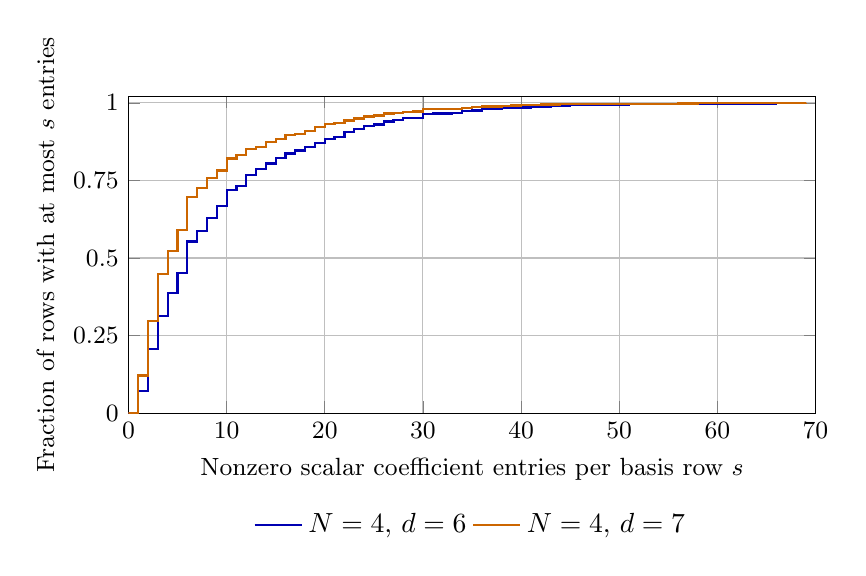
\begin{tikzpicture}
\begin{axis}[width=.85\textwidth,height=5.6cm,xmin=0,xmax=70,ymin=0,ymax=1.02,
xlabel={Nonzero scalar coefficient entries per basis row $s$},
ylabel={Fraction of rows with at most $s$ entries},
ytick={0,.25,.5,.75,1},grid=major,
legend style={at={(.5,-.28)},anchor=north,legend columns=2,draw=none},
tick label style={font=\small},label style={font=\small}]
\addplot+[const plot,no marks,thick,color=blue!70!black] coordinates {(0,0.000000000000) (1,0.072440213606) (2,0.207298196734) (3,0.312901478214) (4,0.386309109202) (5,0.451242163919) (6,0.553091865955) (7,0.586138843743) (8,0.629595232567) (9,0.668291927869) (10,0.719332868973) (11,0.731328844517) (12,0.768709852179) (13,0.786394241932) (14,0.804465598638) (15,0.821414751180) (16,0.837125609473) (17,0.846412816345) (18,0.856744833991) (19,0.869863013699) (20,0.884451667828) (21,0.890527048990) (22,0.905696153548) (23,0.916299048061) (24,0.925547558239) (25,0.930113768284) (26,0.940252302453) (27,0.943696308335) (28,0.951629130872) (29,0.952441761474) (30,0.964708613884) (31,0.965521244486) (32,0.965869514743) (33,0.967262595774) (34,0.973879730671) (35,0.975737172046) (36,0.979916415138) (37,0.980032505224) (38,0.984792198746) (39,0.985372649176) (40,0.985372649176) (41,0.987462270722) (42,0.988507081495) (43,0.990596703042) (44,0.991641513815) (45,0.993731135361) (46,0.994079405619) (47,0.994775946134) (48,0.994775946134) (49,0.994775946134) (50,0.994775946134) (51,0.995820756907) (52,0.995820756907) (53,0.995820756907) (54,0.995820756907) (55,0.995820756907) (56,0.996865567681) (57,0.996865567681) (58,0.997910378454) (59,0.997910378454) (60,0.997910378454) (61,0.997910378454) (62,0.997910378454) (63,0.997910378454) (64,0.997910378454) (65,0.997910378454) (66,0.998955189227) (67,0.998955189227) (68,0.998955189227) (69,1.000000000000)};
\addlegendentry{$N=4$, $d=6$}
\addplot+[const plot,no marks,thick,color=orange!80!black] coordinates {(0,0.000000000000) (1,0.121195577999) (2,0.297029252536) (3,0.447158909968) (4,0.523474819162) (5,0.591033165006) (6,0.697056548838) (7,0.724625813202) (8,0.756949183386) (9,0.782198262135) (10,0.820549565534) (11,0.831490832992) (12,0.850302534007) (13,0.858582412083) (14,0.872799235704) (15,0.884491151449) (16,0.895659888085) (17,0.900868932260) (18,0.909581001774) (19,0.921227423684) (20,0.931099586006) (21,0.935239525044) (22,0.942882489423) (23,0.949888540103) (24,0.956030207907) (25,0.959396751740) (26,0.965606660298) (27,0.967722123652) (28,0.971702834266) (29,0.972044038033) (30,0.979664255493) (31,0.980483144534) (32,0.980551385287) (33,0.981165552068) (34,0.984645830490) (35,0.985737682544) (36,0.988194349666) (37,0.988262590419) (38,0.991060461307) (39,0.991401665074) (40,0.992629998635) (41,0.993858332196) (42,0.995086665757) (43,0.995086665757) (44,0.995700832537) (45,0.996314999318) (46,0.996519721578) (47,0.996929166098) (48,0.996929166098) (49,0.996929166098) (50,0.996929166098) (51,0.997543332878) (52,0.997543332878) (53,0.997543332878) (54,0.997543332878) (55,0.997543332878) (56,0.998157499659) (57,0.998157499659) (58,0.998771666439) (59,0.998771666439) (60,0.998771666439) (61,0.998771666439) (62,0.998771666439) (63,0.998771666439) (64,0.998771666439) (65,0.998771666439) (66,0.999385833220) (67,0.999385833220) (68,0.999385833220) (69,1.000000000000)};
\addlegendentry{$N=4$, $d=7$}
\end{axis}
\end{tikzpicture}
% END GENERATED SPARSITY
\caption{Cumulative coefficient counts for the local bases on $N=4$.
The full histograms are normalized by their own basis dimensions, with
the same scalar-entry-budget axis and no subsampling or clipping of
counts. The curves describe sparsity of the chosen Bernstein
representations; they do not measure accuracy or solver convergence.}
\label{fig:sparsity}
\end{figure}

\noindent\begin{minipage}{\textwidth}
The accompanying \texttt{src} package, \texttt{test} suite and
\texttt{numerical\_case} scripts reproduce the certificate checks,
Table~\ref{tab:cases} and Figure~\ref{fig:sparsity}. Compact count
summaries and vector figures are retained with the code. Full generated
matrices, command logs, input hashes and environment manifests are kept
in local result directories and regenerated by the documented commands.
Thus the distributed finite witnesses suffice to verify the theorem
without retaining every generated numerical basis.
\end{minipage}\par

Algebraic locality leaves a quantitative question: can a decomposition
in \eqref{eq:decomposition} be chosen with a bound uniform in $N$ in
a suitable potential norm? Coefficient sparsity alone does not provide
such a bound. That estimate and its use in multigrid require further analysis.

\begin{thebibliography}{9}
\bibitem{FMS}
P.~E. Farrell, L.~Mitchell and L.~R. Scott,
\emph{Two conjectures on the Stokes complex in three dimensions on
Freudenthal meshes}, SIAM Journal on Scientific Computing
\textbf{46}(2) (2024), A629--A644.
\href{https://doi.org/10.1137/22M1533943}{doi:10.1137/22M1533943}.
Primary text: \href{https://arxiv.org/abs/2211.05494v2}{arXiv:2211.05494v2}.

\bibitem{DMYZ}
S.~Ding, P.~Ming, H.~Yu and Q.~Zhu,
\emph{The Scott--Vogelius element is inf-sup stable on Freudenthal meshes
for $k\ge4$}, preprint, 22 September 2026.
\href{https://arxiv.org/abs/2609.25690v1}{arXiv:2609.25690v1}.
\end{thebibliography}

\section*{AI-use declaration}
ChatGPT assisted with the candidate construction and certificate-producing
code. Codex assisted with the expanded proof, reference verification,
implementation, tests and manuscript preparation. All reported finite
certificate checks and construction cases were replayed from the saved
data; no proof-assistant verification or independent human review is claimed.

\end{document}
